% --- LaTeX Presentation Template - S. Venkatraman ---

% --- Set document class ---

% Remove "handout" when presenting to include pauses
\documentclass[aspectratio=169, dvipsnames, handout]{beamer}
\usetheme{default}

% Make content that is hidden by pauses "transparent"
\setbeamercovered{transparent}

% --- Slide layout settings ---

% Set line spacing
\renewcommand{\baselinestretch}{1.15}

% Set left and right text margins
\setbeamersize{text margin left=12mm, text margin right=12mm}

% Footline: custom author | title | slide numbers
% (replaces the default frame number footline)

% Remove navigation symbols
\setbeamertemplate{navigation symbols}{}

% Allow local line spacing changes
\usepackage{setspace}

% Change itemized list bullets to circles
\setbeamertemplate{itemize item}{$\bullet$}
\setbeamertemplate{itemize subitem}{$\circ$}

% --- Color and font settings ---

\usepackage{xcolor}
\usepackage{graphicx}
\usepackage{subfigure}
\usepackage{booktabs}
\usepackage{multirow}
\usepackage{algorithm}
\usepackage{algpseudocode}
\usepackage{float}
\usepackage{natbib}
\usepackage{amsmath, amsfonts, amssymb}
\usepackage{dsfont}
\usepackage{tikz}

% Bibliography style (used if citations are present)
\bibliographystyle{plain}

% Slide title background color
\definecolor{background}{HTML}{ede6d8}

% Slide title text color
\definecolor{titleText}{HTML}{B40404}

% Other possible color schemes

% - Light green/dark green -
%\definecolor{background}{HTML}{e4ede4}
%\definecolor{titleText}{HTML}{2e592f}

% - Light blue/dark blue -
%\definecolor{background}{HTML}{d5d9e8}
%\definecolor{titleText}{HTML}{2d375e}

% - Beige/dark blue -
%\definecolor{background}{HTML}{e8e2d5}
%\definecolor{titleText}{HTML}{2d3375}

% Set colors
\setbeamercolor{frametitle}{bg=background, fg=titleText}
\setbeamercolor{subtitle}{fg=titleText}

% Set font sizes for frame title and subtitle
\setbeamerfont{frametitle}{size=\fontsize{15}{16}}
\setbeamerfont{framesubtitle}{size=\small}

% --- Custom footline (author | title | slide numbers) ---
\defbeamertemplate{footline}{NGEGFootlineTemplate}{%
    \leavevmode
    \hbox{%
        \begin{beamercolorbox}[wd=.2\paperwidth,ht=2.25ex,dp=1ex,center]{author in head/foot}%
            \ifnum \the\value{page}>1 \usebeamerfont{author in head/foot}\insertshortauthor\fi
        \end{beamercolorbox}%
        \begin{beamercolorbox}[wd=.6\paperwidth,ht=2.25ex,dp=1ex,center]{title in head/foot}%
            \ifnum \the\value{page}>1 \usebeamerfont{title in head/foot}\insertshorttitle\fi
        \end{beamercolorbox}%
        \begin{beamercolorbox}[wd=0.2\paperwidth,ht=2.25ex,dp=1ex,center]{author in head/foot}%
            \ifnum \the\value{page}>1 \insertframenumber{} / \inserttotalframenumber\fi
        \end{beamercolorbox}}
}
\setbeamertemplate{footline}[NGEGFootlineTemplate]

% --- Math/Statistics commands ---

% Add a reference number to a single line of a multi-line equation
% Usage: "\numberthis\label{labelNameHere}" in an align or gather environment
\newcommand\numberthis{\addtocounter{equation}{1}\tag{\theequation}}

% Shortcut for bold text in math mode, e.g. $\b{X}$
\let\b\mathbf

% Shortcut for bold Greek letters, e.g. $\bg{\beta}$
\let\bg\boldsymbol

% Shortcut for calligraphic script, e.g. %\mc{M}$
\let\mc\mathcal

% \mathscr{(letter here)} is sometimes used to denote vector spaces
\usepackage[mathscr]{euscript}

% Convergence: right arrow with optional text on top
% E.g. $\converge[p]$ for converges in probability
\newcommand{\converge}[1][]{\xrightarrow{#1}}

% Weak convergence: harpoon symbol with optional text on top
% E.g. $\wconverge[n\to\infty]$
\newcommand{\wconverge}[1][]{\stackrel{#1}{\rightharpoonup}}

% Equality: equals sign with optional text on top
% E.g. $X \equals[d] Y$ for equality in distribution
\newcommand{\equals}[1][]{\stackrel{\smash{#1}}{=}}

% Normal distribution: arguments are the mean and variance
% E.g. $\normal{\mu}{\sigma}$
\newcommand{\normal}[2]{\mathcal{N}\left(#1,#2\right)}

% Uniform distribution: arguments are the left and right endpoints
% E.g. $\unif{0}{1}$
\newcommand{\unif}[2]{\text{Uniform}(#1,#2)}

% Independent and identically distributed random variables
% E.g. $ X_1,...,X_n \iid \normal{0}{1}$
\newcommand{\iid}{\stackrel{\smash{\text{iid}}}{\sim}}

% Sequences (this shortcut is mostly to reduce finger strain for small hands)
% E.g. to write $\{A_n\}_{n\geq 1}$, do $\bk{A_n}{n\geq 1}$
\newcommand{\bk}[2]{\{#1\}_{#2}}

% Math mode symbols for common sets and spaces. Example usage: $\R$
\newcommand{\R}{\mathbb{R}}	% Real numbers
\newcommand{\D}{\mathbb{D}}	% Complex numbers
\newcommand{\Q}{\mathbb{Q}}	% Rational numbers
\newcommand{\Z}{\mathbb{Z}}	% Integers
\newcommand{\N}{\mathbb{N}}	% Natural numbers
\newcommand{\F}{\mathcal{F}}	% Calligraphic F for a sigma algebra
\newcommand{\El}{\mathcal{L}}	% Calligraphic L, e.g. for L^p spaces

% Math mode symbols for probability
\newcommand{\pr}{\mathbb{P}}	% Probability measure
\newcommand{\E}{\mathbb{E}}	% Expectation, e.g. $\E(X)$
\newcommand{\var}{\text{Var}}	% Variance, e.g. $\var(X)$
\newcommand{\cov}{\text{Cov}}	% Covariance, e.g. $\cov(X,Y)$
\newcommand{\corr}{\text{Corr}}	% Correlation, e.g. $\corr(X,Y)$
\newcommand{\B}{\mathcal{B}}	% Borel sigma-algebra

% Other miscellaneous symbols
\newcommand{\tth}{\text{th}}	% Non-italicized 'th', e.g. $n^\tth$
\newcommand{\Oh}{\mathcal{O}}	% Big-O notation, e.g. $\O(n)$
\newcommand{\1}{\mathds{1}}	% Indicator function, e.g. $\1_A$
\providecommand{\Vec}[1]{\boldsymbol{#1}} % Bold vector helper

% Additional commands for math mode
\DeclareMathOperator*{\argmax}{argmax}	% Argmax, e.g. $\argmax_{x\in[0,1]} f(x)$
\DeclareMathOperator*{\argmin}{argmin}	% Argmin, e.g. $\argmin_{x\in[0,1]} f(x)$
\DeclareMathOperator*{\spann}{Span}	% Span, e.g. $\spann\{X_1,...,X_n\}$
\DeclareMathOperator*{\bias}{Bias}	% Bias, e.g. $\bias(\hat\theta)$
\DeclareMathOperator*{\ran}{ran}		% Range of an operator, e.g. $\ran(T) 
\DeclareMathOperator*{\dv}{d\!}		% Non-italicized 'with respect to', e.g. $\int f(x) \dv x$
\DeclareMathOperator*{\diag}{diag}	% Diagonal of a matrix, e.g. $\diag(M)$
\DeclareMathOperator*{\trace}{trace}	% Trace of a matrix, e.g. $\trace(M)$
\DeclareMathOperator*{\supp}{supp}	% Support of a function, e.g., $\supp(f)$

% --- Unified paper intro slide macro ---
% Usage: \PaperIntro{Frame Heading}{Paper Title}{Authors}{Footnote}
\newcommand{\PaperIntro}[4]{%
\begin{frame}[plain]{#1}
    \centering
    {\Large #2}\\[6pt]
    {\small #3}\\[4pt]
    {\footnotesize #4}
\end{frame}
}

% --- Document metadata ---
\title[Short Title]{Your Presentation Title}
\author[Your Name]{Your Name}
\date{\today} % Or specify date

\begin{document}

% --- Title slide ---
\begin{frame}
    \titlepage
\end{frame}

% --- Outline slide ---
\section*{Outline}
\begin{frame}{Outline}
    \tableofcontents[hideallsubsections]
\end{frame}

% --- Section 1 ---
\section{Introduction}

\begin{frame}{Introduction Slide}
    \begin{itemize}
        \item First point
        \item Second point
        \item Third point
    \end{itemize}
\end{frame}

\begin{frame}{Example with Figure}
    \centering
    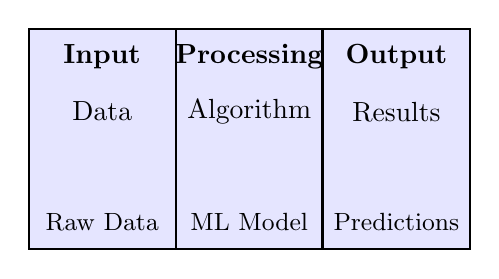
\begin{tikzpicture}[scale=0.7]
        % Draw a simple framework diagram
        \draw[thick, fill=blue!10] (0,0) rectangle (8,4);
        \draw[thick] (2.67,0) -- (2.67,4);
        \draw[thick] (5.33,0) -- (5.33,4);

        % Add labels
        \node[font=\bfseries] at (1.33,3.5) {Input};
        \node[font=\bfseries] at (4,3.5) {Processing};
        \node[font=\bfseries] at (6.67,3.5) {Output};

        % Add components
        \node at (1.33,2.5) {Data};
        \node at (4,2.5) {Algorithm};
        \node at (6.67,2.5) {Results};

        % Add bottom elements
        \node[font=\small] at (1.33,0.5) {Raw Data};
        \node[font=\small] at (4,0.5) {ML Model};
        \node[font=\small] at (6.67,0.5) {Predictions};
    \end{tikzpicture}
    \vspace{2pt}

    {\small Example framework diagram generated with TikZ.}
\end{frame}

% --- Section 2 ---
\section{Main Content}

\subsection{Subsection Example}

\begin{frame}{Subsection Slide}
    \begin{itemize}
        \item Point A
        \item Point B
        \item Point C
    \end{itemize}
\end{frame}

\begin{frame}{Mathematical Content}
    \begin{itemize}
        \item Example equation: $y = mx + b$
        \item Probability notation: $\pr(X > 0)$
        \item Expectation: $\E[X]$
    \end{itemize}
\end{frame}

\begin{frame}{Two-Column Layout}
    \begin{columns}
        \begin{column}{0.48\textwidth}
            \textbf{Left Column}
            \begin{itemize}
                \item Item 1
                \item Item 2
            \end{itemize}
        \end{column}
        \begin{column}{0.48\textwidth}
            \textbf{Right Column}
            \begin{itemize}
                \item Item A
                \item Item B
            \end{itemize}
        \end{column}
    \end{columns}
\end{frame}

% --- Section 3 ---
\section{Results}

\begin{frame}{Results Overview}
    \begin{itemize}
        \item Result 1
        \item Result 2
        \item Result 3
    \end{itemize}
\end{frame}

\begin{frame}{Table Example}
    \centering
    \begin{tabular}{lcc}
        \toprule
        \textbf{Method} & \textbf{Metric 1} & \textbf{Metric 2} \\
        \midrule
        Method A & 0.85 & 0.92 \\
        Method B & 0.80 & 0.88 \\
        \textbf{Ours} & \textbf{0.90} & \textbf{0.95} \\
        \bottomrule
    \end{tabular}
\end{frame}

% --- Conclusion ---
\section{Conclusion}

\begin{frame}{Conclusion}
    \begin{itemize}
        \item Summary point 1
        \item Summary point 2
        \item Future work
    \end{itemize}
\end{frame}

% --- Thank you slide ---
\begin{frame}[plain]
    \centering
    \vspace{1.5cm}
    {\Huge Thank You!}\\[1cm]
    {\Large Questions?}\\[1cm]
    {\small Contact: your.email@domain.com}
\end{frame}

\end{document}
